% ---------
% --------
%!TEX TS-program = pdflatex
%!TEX encoding = UTF-8 Unicode
%!TEX spellcheck = English (Aspell)

\documentclass[11pt]{article}
\usepackage{lucy,handout,graphicx}
\usepackage{tikz}
\usepackage{fourier-orns}
\usepackage{mathtools}
\usepackage[normalem]{ulem} % either use this (simple) or
\pagestyle{empty}

\allowdisplaybreaks

\begin{document}


\begin{center}
\Large\textbf{CSCI 332, Fall 2026}%
\\
\LARGE\textbf{In-class Activity}%
\end{center}

In this activity, you will trace through the algorithm whatever-first-search. 

\begin{verbatim}
WFS(s):
	put s into the bag
	while the bag is not empty:
		take v from the bag
		if v is unmarked:
			mark v
			for each edge {v,w}:
				put w into the bag
\end{verbatim}

Complete the trace of $WFS(a)$ on the graph below. Remove from the bag in \EMPH{alphabetical order}.

\begin{center}
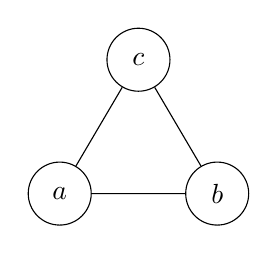
\begin{tikzpicture}[every node/.style={circle,draw,minimum size=8mm}]
	\node (a) at (0,0) {$a$};
	\node (b) at (2,0) {$b$};
	\node (c) at (1,1.7) {$c$};
	\draw (a) -- (b) -- (c) -- (a);
\end{tikzpicture}
\end{center}

\begin{center}
\small
{\renewcommand{\arraystretch}{1.8}
\begin{tabular}{|c|c|p{5.2cm}|p{3.2cm}|}
\hline
After iteration & Took out of bag & Bag & verts that have been marked \\

\hline
0 & -- & a & -- \\ \hline
1 & $a$ & $b,c$ & $a$ \\ \hline
2 & \hspace{.4in} & \hspace{.4in} & \hspace{.4in} \\ \hline
3 & \hspace{.4in} & \hspace{.4in} & \hspace{.4in} \\ \hline
4 & \hspace{.4in} & \hspace{.4in} & \hspace{.4in} \\ \hline
5 & \hspace{.4in} & \hspace{.4in} & \hspace{.4in} \\ \hline
6 & \hspace{.4in} & \hspace{.4in} & \hspace{.4in} \\ \hline
7 & \hspace{.4in} & \hspace{.4in} & \hspace{.4in} \\ \hline
\end{tabular}
}
\end{center}


%%%%%%%%%%%%%%%%%%%%
\end{document}
